\documentclass{standalone}
\usepackage{tikz}
\usetikzlibrary{patterns, positioning}


\begin{document}
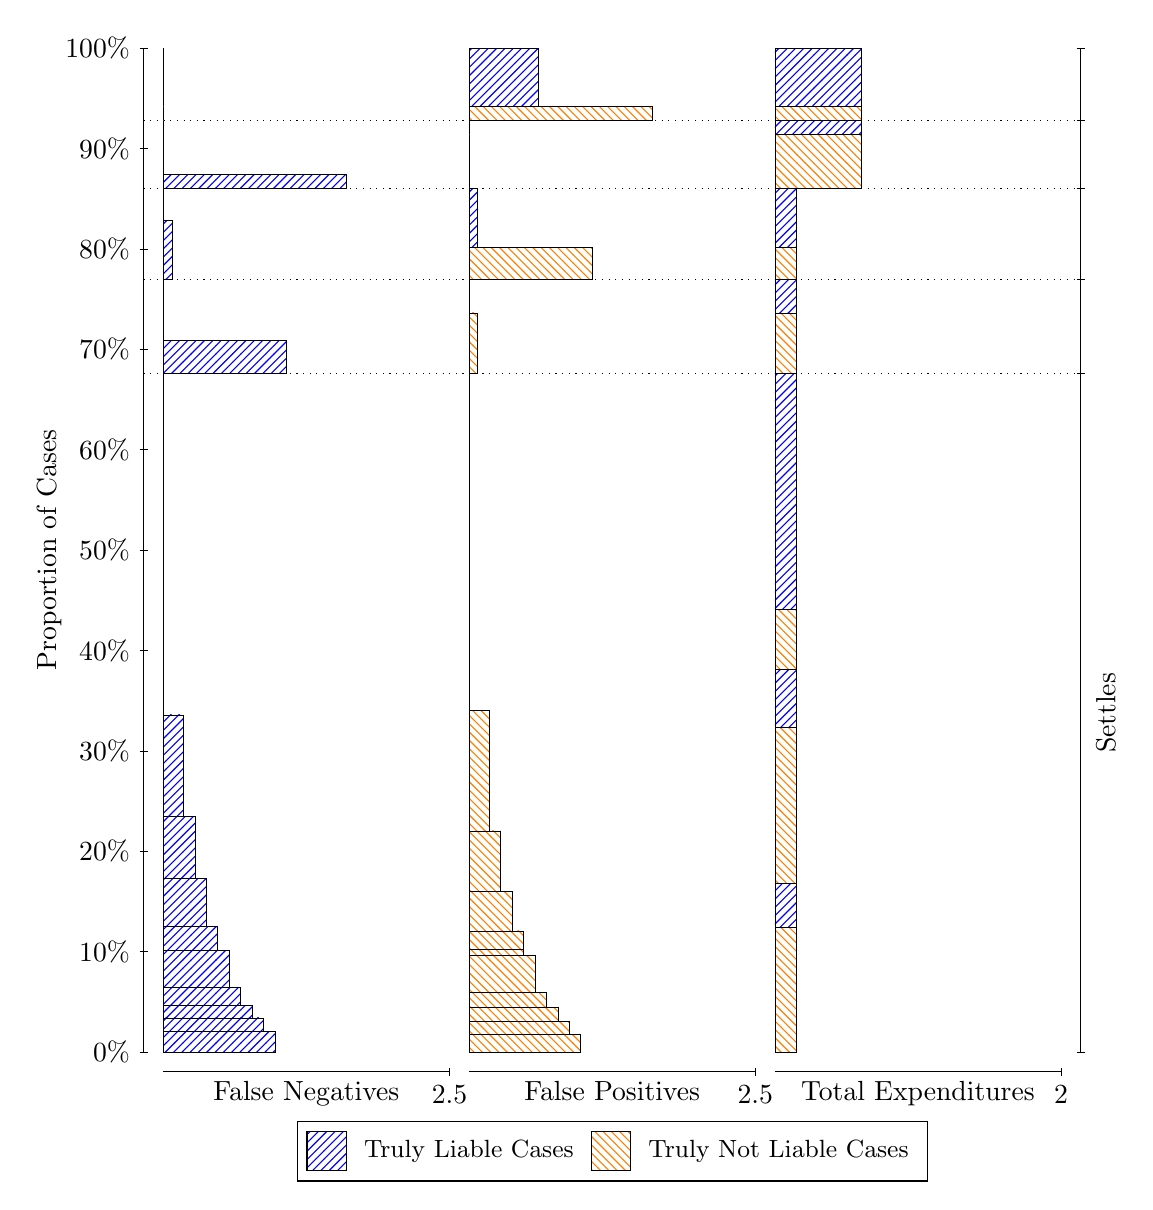
\begin{tikzpicture}
\draw[black, very thin] (1.5,1.75) -- (1.5,14.5);
\node[rotate=90, text=black, anchor=center] at (0.3, 8.125) {Proportion of Cases};
\draw[black, very thin] (1.45,1.75) -- (1.55,1.75);
\node[text=black, anchor=east] at (1.45, 1.75) {0\%};
\draw[black, very thin] (1.45,3.025) -- (1.55,3.025);
\node[text=black, anchor=east] at (1.45, 3.025) {10\%};
\draw[black, very thin] (1.45,4.3) -- (1.55,4.3);
\node[text=black, anchor=east] at (1.45, 4.3) {20\%};
\draw[black, very thin] (1.45,5.575) -- (1.55,5.575);
\node[text=black, anchor=east] at (1.45, 5.575) {30\%};
\draw[black, very thin] (1.45,6.85) -- (1.55,6.85);
\node[text=black, anchor=east] at (1.45, 6.85) {40\%};
\draw[black, very thin] (1.45,8.125) -- (1.55,8.125);
\node[text=black, anchor=east] at (1.45, 8.125) {50\%};
\draw[black, very thin] (1.45,9.4) -- (1.55,9.4);
\node[text=black, anchor=east] at (1.45, 9.4) {60\%};
\draw[black, very thin] (1.45,10.675) -- (1.55,10.675);
\node[text=black, anchor=east] at (1.45, 10.675) {70\%};
\draw[black, very thin] (1.45,11.95) -- (1.55,11.95);
\node[text=black, anchor=east] at (1.45, 11.95) {80\%};
\draw[black, very thin] (1.45,13.225) -- (1.55,13.225);
\node[text=black, anchor=east] at (1.45, 13.225) {90\%};
\draw[black, very thin] (1.45,14.5) -- (1.55,14.5);
\node[text=black, anchor=east] at (1.45, 14.5) {100\%};

\draw[black, very thin] (13.4,1.75) -- (13.4,14.5);
\draw[black, very thin] (13.35,1.75) -- (13.45,1.75);
\node[anchor=west] at (13.35, 1.75) {};
\draw[black, very thin] (13.35,10.364) -- (13.45,10.364);
\node[anchor=west] at (13.35, 10.364) {};
\draw[black, very thin] (13.35,11.564) -- (13.45,11.564);
\node[anchor=west] at (13.35, 11.564) {};
\draw[black, very thin] (13.35,12.719) -- (13.45,12.719);
\node[anchor=west] at (13.35, 12.719) {};
\draw[black, very thin] (13.35,13.582) -- (13.45,13.582);
\node[anchor=west] at (13.35, 13.582) {};
\draw[black, very thin] (13.35,14.5) -- (13.45,14.5);
\node[anchor=west] at (13.35, 14.5) {};

\draw[black, very thin, pattern color=blue, pattern=north east lines] (1.75,1.75) rectangle (3.167,2.0135);
\draw[black, very thin, pattern color=blue, pattern=north east lines] (1.75,2.0135) rectangle (3.0217,2.1829);
\draw[black, very thin, pattern color=blue, pattern=north east lines] (1.75,2.1829) rectangle (2.8763,2.34);
\draw[black, very thin, pattern color=blue, pattern=north east lines] (1.75,2.34) rectangle (2.731,2.5672);
\draw[black, very thin, pattern color=blue, pattern=north east lines] (1.75,2.5672) rectangle (2.5857,3.037);
\draw[black, very thin, pattern color=blue, pattern=north east lines] (1.75,3.037) rectangle (2.4403,3.3461);
\draw[black, very thin, pattern color=blue, pattern=north east lines] (1.75,3.3461) rectangle (2.295,3.9501);
\draw[black, very thin, pattern color=blue, pattern=north east lines] (1.75,3.9501) rectangle (2.1497,4.7433);
\draw[black, very thin, pattern color=blue, pattern=north east lines] (1.75,4.7433) rectangle (2.0043,6.0302);
\draw[black, very thin, pattern color=orange, pattern=north west lines] (1.75,6.0302) rectangle (1.75,10.364);
\draw[black, very thin, pattern color=blue, pattern=north east lines] (1.75,10.364) rectangle (3.3123,10.79);
\draw[black, very thin, pattern color=orange, pattern=north west lines] (1.75,10.79) rectangle (1.75,11.564);
\draw[black, very thin, pattern color=blue, pattern=north east lines] (1.75,11.564) rectangle (1.859,12.314);
\draw[black, very thin, pattern color=orange, pattern=north west lines] (1.75,12.314) rectangle (1.75,12.719);
\draw[black, very thin, pattern color=blue, pattern=north east lines] (1.75,12.719) rectangle (4.0753,12.897);
\draw[black, very thin, pattern color=orange, pattern=north west lines] (1.75,12.897) rectangle (1.75,13.582);
\draw[black, very thin, pattern color=orange, pattern=north west lines] (1.75,13.582) rectangle (1.75,13.76);
\draw[black, very thin, pattern color=blue, pattern=north east lines] (1.75,13.76) rectangle (1.75,14.5);
\draw[black, very thin, pattern color=orange, pattern=north west lines] (5.6333,1.75) rectangle (7.0503,1.9751);
\draw[black, very thin, pattern color=orange, pattern=north west lines] (5.6333,1.9751) rectangle (6.905,2.1417);
\draw[black, very thin, pattern color=orange, pattern=north west lines] (5.6333,2.1417) rectangle (6.7597,2.3142);
\draw[black, very thin, pattern color=orange, pattern=north west lines] (5.6333,2.3142) rectangle (6.6143,2.5113);
\draw[black, very thin, pattern color=orange, pattern=north west lines] (5.6333,2.5113) rectangle (6.469,2.9729);
\draw[black, very thin, pattern color=orange, pattern=north west lines] (5.6333,2.9729) rectangle (6.3237,3.0504);
\draw[black, very thin, pattern color=orange, pattern=north west lines] (5.6333,3.0504) rectangle (6.3237,3.2883);
\draw[black, very thin, pattern color=orange, pattern=north west lines] (5.6333,3.2883) rectangle (6.1783,3.7878);
\draw[black, very thin, pattern color=orange, pattern=north west lines] (5.6333,3.7878) rectangle (6.033,4.5573);
\draw[black, very thin, pattern color=orange, pattern=north west lines] (5.6333,4.5573) rectangle (5.8877,6.0833);
\draw[black, very thin, pattern color=blue, pattern=north east lines] (5.6333,6.0833) rectangle (5.6333,10.364);
\draw[black, very thin, pattern color=orange, pattern=north west lines] (5.6333,10.364) rectangle (5.7423,11.137);
\draw[black, very thin, pattern color=blue, pattern=north east lines] (5.6333,11.137) rectangle (5.6333,11.564);
\draw[black, very thin, pattern color=orange, pattern=north west lines] (5.6333,11.564) rectangle (7.1957,11.969);
\draw[black, very thin, pattern color=blue, pattern=north east lines] (5.6333,11.969) rectangle (5.7423,12.719);
\draw[black, very thin, pattern color=orange, pattern=north west lines] (5.6333,12.719) rectangle (5.6333,13.403);
\draw[black, very thin, pattern color=blue, pattern=north east lines] (5.6333,13.403) rectangle (5.6333,13.582);
\draw[black, very thin, pattern color=orange, pattern=north west lines] (5.6333,13.582) rectangle (7.9587,13.76);
\draw[black, very thin, pattern color=blue, pattern=north east lines] (5.6333,13.76) rectangle (6.5053,14.5);
\draw[black, very thin, pattern color=orange, pattern=north west lines] (9.5167,1.75) rectangle (9.7892,3.3344);
\draw[black, very thin, pattern color=blue, pattern=north east lines] (9.5167,3.3344) rectangle (9.7892,3.8881);
\draw[black, very thin, pattern color=orange, pattern=north west lines] (9.5167,3.8881) rectangle (9.7892,5.8757);
\draw[black, very thin, pattern color=blue, pattern=north east lines] (9.5167,5.8757) rectangle (9.7892,6.609);
\draw[black, very thin, pattern color=orange, pattern=north west lines] (9.5167,6.609) rectangle (9.7892,7.3703);
\draw[black, very thin, pattern color=blue, pattern=north east lines] (9.5167,7.3703) rectangle (9.7892,10.364);
\draw[black, very thin, pattern color=orange, pattern=north west lines] (9.5167,10.364) rectangle (9.7892,11.137);
\draw[black, very thin, pattern color=blue, pattern=north east lines] (9.5167,11.137) rectangle (9.7892,11.564);
\draw[black, very thin, pattern color=orange, pattern=north west lines] (9.5167,11.564) rectangle (9.7892,11.969);
\draw[black, very thin, pattern color=blue, pattern=north east lines] (9.5167,11.969) rectangle (9.7892,12.719);
\draw[black, very thin, pattern color=orange, pattern=north west lines] (9.5167,12.719) rectangle (10.607,13.403);
\draw[black, very thin, pattern color=blue, pattern=north east lines] (9.5167,13.403) rectangle (10.607,13.582);
\draw[black, very thin, pattern color=orange, pattern=north west lines] (9.5167,13.582) rectangle (10.607,13.76);
\draw[black, very thin, pattern color=blue, pattern=north east lines] (9.5167,13.76) rectangle (10.607,14.5);
\draw[black, dotted] (1.5,10.364) -- (13.4,10.364);
\draw[black, dotted] (1.5,11.564) -- (13.4,11.564);
\draw[black, dotted] (1.5,12.719) -- (13.4,12.719);
\draw[black, dotted] (1.5,13.582) -- (13.4,13.582);
\draw[black, very thin] (1.75,1.5) -- (5.3833,1.5);
\node[text=black, anchor=north] at (3.5667, 1.5) {False Negatives};
\draw[black, very thin] (5.3833,1.45) -- (5.3833,1.55);
\node[text=black, anchor=north] at (5.3833, 1.45) {2.5};

\draw[black, very thin] (5.6333,1.5) -- (9.2667,1.5);
\node[text=black, anchor=north] at (7.45, 1.5) {False Positives};
\draw[black, very thin] (9.2667,1.45) -- (9.2667,1.55);
\node[text=black, anchor=north] at (9.2667, 1.45) {2.5};

\draw[black, very thin] (9.5167,1.5) -- (13.15,1.5);
\node[text=black, anchor=north] at (11.333, 1.5) {Total Expenditures};
\draw[black, very thin] (13.15,1.45) -- (13.15,1.55);
\node[text=black, anchor=north] at (13.15, 1.45) {2};

\node[text=black, centered, rotate=90] at (13.72, 6.0568) {Settles};





\draw (7.449999999999999,1.5) node[draw=none] (baseCoordinate) {};
\begin{scope}[align=center]
        \matrix[scale=0.5, draw=black, below=0.5cm of baseCoordinate, nodes={draw}, column sep=0.1cm]{
            \node[rectangle, draw, minimum width=0.5cm, minimum height=0.5cm, pattern color=blue, pattern=north east lines] {}; &
            \node[draw=none, font=\small, text=black] (B) {Truly Liable Cases}; &
            \node[rectangle, draw, minimum width=0.5cm, minimum height=0.5cm, pattern color=orange, pattern=north west lines] {}; &
            \node[draw=none, font=\small, text=black] (B) {Truly Not Liable Cases}; \\
            };
\end{scope}

\end{tikzpicture}
\end{document}